% ============================================================
\chapter{Linear Programming --- Formulation and Geometry}
\label{ch:linear_programming}
% ============================================================

In the summer of 1947, at the Pentagon, a young mathematician named George Dantzig was working on planning problems for the United States Air Force. Resources were scarce, constraints were everywhere, and the objective was clear: do the most with the least. Dantzig formalised this challenge as a \emph{linear program} and invented the simplex algorithm to solve it. Within months, the method was tackling logistics, diet planning, and industrial scheduling problems that had seemed intractable.

What makes linear programming so remarkable is the marriage of algebra and geometry. A linear program defines a convex polyhedron in high-dimensional space, and the optimal solution---if it exists---sits at a vertex of this polyhedron. The simplex algorithm simply walks from vertex to vertex along the edges, improving the objective at each step. This geometric insight, combined with the power of duality theory developed shortly after by John von Neumann, turned linear programming into one of the most widely used tools in all of applied mathematics.

\section{General form of a linear program}

\begin{definition}[Linear program]
A \textbf{linear program} (LP) is an optimization problem of the form:
\[
\begin{aligned}
  \min \quad & \mathbf{c}^\top \mathbf{x} \\
  \text{s.t.} \quad
    & A\mathbf{x} \le \mathbf{b} \\
    & \mathbf{x} \ge \mathbf{0}
\end{aligned}
\]
where $\mathbf{c} \in \R^n$, $A \in \R^{m \times n}$, $\mathbf{b} \in \R^m$,
and $\mathbf{x} \in \R^n$ is the vector of decision variables.
\end{definition}

\begin{remark}
Maximizing $\mathbf{c}^\top \mathbf{x}$ is equivalent to minimizing
$(-\mathbf{c})^\top \mathbf{x}$.  Hence we can always convert to a
minimization problem.
\end{remark}

\section{Equivalent forms}

\subsection{Standard form}

\begin{definition}[Standard form]
An LP is in \textbf{standard form} if:
\[
\begin{aligned}
  \min \quad & \mathbf{c}^\top \mathbf{x} \\
  \text{s.t.} \quad
    & A\mathbf{x} = \mathbf{b} \\
    & \mathbf{x} \ge \mathbf{0}
\end{aligned}
\]
All constraints are equalities and all variables are nonnegative.
\end{definition}

\subsection{Converting to standard form}

\begin{keyformulas}[title=\textbf{Conversion rules}]
\begin{enumerate}
  \item \textbf{$\le$ inequality}: add a slack variable $s_i \ge 0$:
        \[a_{i1}x_1 + \cdots + a_{in}x_n + s_i = b_i\]
  \item \textbf{$\ge$ inequality}: subtract a surplus variable $s_i \ge 0$:
        \[a_{i1}x_1 + \cdots + a_{in}x_n - s_i = b_i\]
  \item \textbf{Free variable} ($x_j \in \R$): set
        $x_j = x_j^+ - x_j^-$ with $x_j^+, x_j^- \ge 0$.
  \item \textbf{Maximization}: $\max \mathbf{c}^\top\mathbf{x} =
        -\min(-\mathbf{c}^\top\mathbf{x})$.
\end{enumerate}
\end{keyformulas}

\begin{example}[Converting to standard form]
Consider:
\[
\begin{aligned}
  \max \quad & 3x_1 + 5x_2 \\
  \text{s.t.} \quad
    & x_1 + 2x_2 \le 12 \\
    & 2x_1 + x_2 \ge 4 \\
    & x_1 \ge 0, \; x_2 \text{ free}
\end{aligned}
\]

Set $x_2 = x_2^+ - x_2^-$ with $x_2^+, x_2^- \ge 0$, and add
slack/surplus variables:
\[
\begin{aligned}
  \min \quad & -3x_1 - 5x_2^+ + 5x_2^- \\
  \text{s.t.} \quad
    & x_1 + 2x_2^+ - 2x_2^- + s_1 = 12 \\
    & 2x_1 + x_2^+ - x_2^- - s_2 = 4 \\
    & x_1, x_2^+, x_2^-, s_1, s_2 \ge 0
\end{aligned}
\]
\end{example}

\section{Canonical form}

\begin{definition}[Canonical form]
An LP is in \textbf{canonical form} if:
\[
\begin{aligned}
  \max \quad & \mathbf{c}^\top \mathbf{x} \\
  \text{s.t.} \quad
    & A\mathbf{x} \le \mathbf{b} \\
    & \mathbf{x} \ge \mathbf{0}
\end{aligned}
\]
(maximization, $\le$ constraints, nonnegative variables).
\end{definition}

\section{Geometry of linear programming}

\subsection{Hyperplanes and half-spaces}

\begin{definition}[Hyperplane]
A \textbf{hyperplane} in $\R^n$ is a set of the form:
\[
  H = \{\mathbf{x} \in \R^n : \mathbf{a}^\top \mathbf{x} = \beta\}
\]
where $\mathbf{a} \in \R^n \setminus \{\mathbf{0}\}$ and $\beta \in \R$.
\end{definition}

\begin{definition}[Half-space]
A \textbf{half-space} is one of the two sets determined by a hyperplane:
\[
  H^+ = \{\mathbf{x} : \mathbf{a}^\top \mathbf{x} \le \beta\}
  \qquad \text{or} \qquad
  H^- = \{\mathbf{x} : \mathbf{a}^\top \mathbf{x} \ge \beta\}
\]
\end{definition}

\subsection{Convex sets and polyhedra}

\begin{definition}[Convex set]
A set $C \subseteq \R^n$ is \textbf{convex} if for all
$\mathbf{x}, \mathbf{y} \in C$ and all $\lambda \in [0,1]$:
\[
  \lambda \mathbf{x} + (1-\lambda)\mathbf{y} \in C
\]
\end{definition}

\begin{definition}[Polyhedron]
A \textbf{polyhedron} is the intersection of finitely many half-spaces:
\[
  P = \{\mathbf{x} \in \R^n : A\mathbf{x} \le \mathbf{b}\}
\]
A bounded polyhedron is called a \textbf{polytope}.
\end{definition}

\begin{theorem}[The feasible set is a polyhedron]
The feasible set of a linear program:
\[
  \mathcal{F} = \{\mathbf{x} \in \R^n : A\mathbf{x} \le \mathbf{b},\;
  \mathbf{x} \ge \mathbf{0}\}
\]
is a convex polyhedron (possibly empty or unbounded).
\end{theorem}

\begin{center}
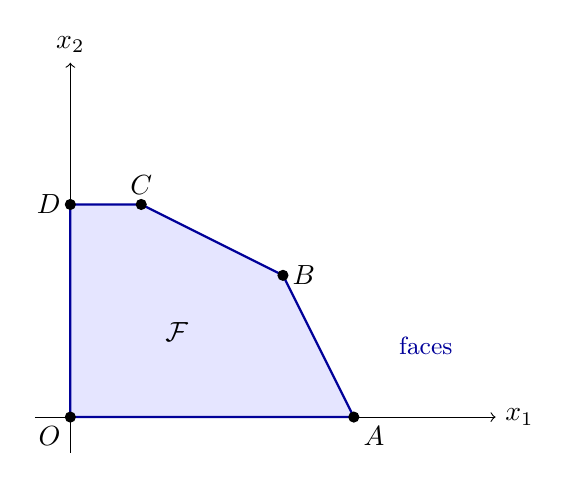
\begin{tikzpicture}[scale=0.9]
  \draw[->] (-0.5,0) -- (6,0) node[right] {$x_1$};
  \draw[->] (0,-0.5) -- (0,5) node[above] {$x_2$};
  % Polyhedron
  \fill[blue!10] (0,0) -- (4,0) -- (3,2) -- (1,3) -- (0,3) -- cycle;
  \draw[thick, blue!60!black] (0,0) -- (4,0) -- (3,2) -- (1,3) -- (0,3) -- cycle;
  % Vertices
  \foreach \point/\name/\posi in
    {(0,0)/O/below left, (4,0)/A/below right,
     (3,2)/B/right, (1,3)/C/above, (0,3)/D/left}
    \filldraw \point circle (2pt) node[\posi] {$\name$};
  \node at (1.5,1.2) {$\mathcal{F}$};
  \node[blue!60!black, right] at (4.5,1) {\small faces};
\end{tikzpicture}
\end{center}

\subsection{Vertices and basic feasible solutions}

\begin{definition}[Vertex]
A point $\mathbf{v} \in P$ is a \textbf{vertex} (or \textbf{extreme point})
of polyhedron $P$ if there do not exist two distinct points
$\mathbf{x}, \mathbf{y} \in P$ such that
$\mathbf{v} = \frac{1}{2}(\mathbf{x} + \mathbf{y})$.
\end{definition}

\begin{definition}[Basic feasible solution (BFS)]
Consider the system $A\mathbf{x} = \mathbf{b}$ with
$A \in \R^{m \times n}$, $m \le n$, $\text{rank}(A) = m$.  Partition the
columns into $B$ (basis, $m$ linearly independent columns) and $N$
(non-basic):
\[
  \mathbf{x}_B = B^{-1}\mathbf{b}, \qquad \mathbf{x}_N = \mathbf{0}
\]
If $\mathbf{x}_B \ge \mathbf{0}$, then $\mathbf{x}$ is a \textbf{basic
feasible solution}.
\end{definition}

\begin{theorem}[Vertex--BFS equivalence]
\label{thm:vertex_bfs}
Let $P = \{\mathbf{x} : A\mathbf{x} = \mathbf{b},\; \mathbf{x} \ge 0\}$.
The following are equivalent:
\begin{enumerate}
  \item $\mathbf{v}$ is a vertex of $P$.
  \item $\mathbf{v}$ is a basic feasible solution.
  \item The columns of $A$ corresponding to the strictly positive components
        of $\mathbf{v}$ are linearly independent.
\end{enumerate}
\end{theorem}

\section{Fundamental theorem of linear programming}

\begin{theorem}[Fundamental theorem of LP]
\label{thm:fundamental_lp}
Consider the LP $\min\{\mathbf{c}^\top\mathbf{x} :
A\mathbf{x} = \mathbf{b},\; \mathbf{x} \ge 0\}$.
\begin{enumerate}
  \item If the feasible set is nonempty, it has at least one vertex.
  \item If the problem has a finite optimal solution, then there exists an
        optimal solution that is a vertex of the feasible set.
  \item The number of vertices is finite (at most $\binom{n}{m}$).
\end{enumerate}
\end{theorem}

\begin{intuition}[title=\textbf{Why is the optimum at a vertex?}]
The level sets of $\mathbf{c}^\top\mathbf{x}$ are parallel hyperplanes.
We slide these hyperplanes in the direction $-\mathbf{c}$ (for minimization)
until they touch the polyhedron.  The last contact point is necessarily a
vertex (or a face containing vertices).
\end{intuition}

\section{Formulation examples}

\begin{example}[Production planning]
A company produces $n$ items on $m$ machines over $T$ periods.
Let $x_{it}$ be the quantity of item $i$ produced in period $t$, and
$s_{it}$ the inventory at the end of the period.

\[
\begin{aligned}
  \min \quad & \sum_{i=1}^{n}\sum_{t=1}^{T}
    (c_{it} x_{it} + h_{it} s_{it}) \\
  \text{s.t.} \quad
    & s_{i,t-1} + x_{it} - s_{it} = d_{it}
      & \forall\, i,t & \quad \text{(flow balance)} \\
    & \sum_{i=1}^{n} a_{ij} x_{it} \le C_{jt}
      & \forall\, j,t & \quad \text{(machine $j$ capacity)} \\
    & x_{it}, s_{it} \ge 0 & \forall\, i,t
\end{aligned}
\]
where $c_{it}$ is unit production cost, $h_{it}$ holding cost, $d_{it}$
demand, $a_{ij}$ unit machine time.
\end{example}

\begin{example}[Diet problem (revisited)]
\label{ex:diet}
With the data from the previous chapter:
\[
\begin{aligned}
  \min \quad & 0.30 x_1 + 0.15 x_2 + 1.20 x_3 + 0.40 x_4 \\
  \text{s.t.} \quad
    & 265 x_1 + 65 x_2 + 350 x_3 + 52 x_4 \ge 2000 \\
    & 9 x_1 + 3.5 x_2 + 25 x_3 + 0.3 x_4 \ge 55 \\
    & 15 x_1 + 120 x_2 + 700 x_3 + 6 x_4 \ge 800 \\
    & x_1, x_2, x_3, x_4 \ge 0
\end{aligned}
\]
(each $x_i$ is in hectograms, i.e., 100\,g).
\end{example}

\section{Detailed graphical solution}

\begin{example}[Complete graphical solution]
Solve:
\[
\begin{aligned}
  \max \quad & z = 2x_1 + 3x_2 \\
  \text{s.t.} \quad
    & x_1 + 2x_2 \le 8 \\
    & 3x_1 + 2x_2 \le 12 \\
    & x_1, x_2 \ge 0
\end{aligned}
\]

\textbf{Step 1}: Plot the constraint lines.
\begin{center}
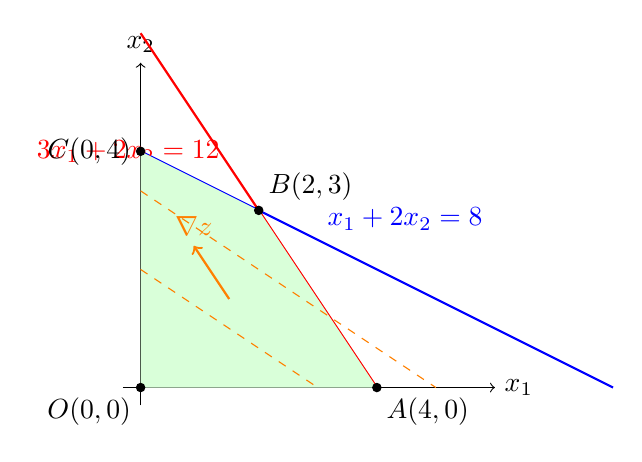
\begin{tikzpicture}[scale=0.75]
  \draw[->] (-0.3,0) -- (6,0) node[right] {$x_1$};
  \draw[->] (0,-0.3) -- (0,5.5) node[above] {$x_2$};
  % Constraints
  \draw[thick, blue] (0,4) -- (8,0);
  \node[blue, above right] at (3,2.5) {$x_1+2x_2=8$};
  \draw[thick, red] (0,6) -- (4,0);
  \node[red, left] at (1.5,4) {$3x_1+2x_2=12$};
  % Feasible region
  \fill[green!15] (0,0) -- (4,0) -- (2,3) -- (0,4) -- cycle;
  % Vertices
  \filldraw (0,0) circle (2pt) node[below left] {$O(0,0)$};
  \filldraw (4,0) circle (2pt) node[below right] {$A(4,0)$};
  \filldraw (2,3) circle (2pt) node[above right] {$B(2,3)$};
  \filldraw (0,4) circle (2pt) node[left] {$C(0,4)$};
  % Level curves
  \draw[dashed, orange] (0,2) -- (3,0);
  \draw[dashed, orange] (0,3.33) -- (5,0);
  \draw[->, orange, thick] (1.5,1.5) -- (0.9,2.4) node[above] {$\nabla z$};
\end{tikzpicture}
\end{center}

\textbf{Step 2}: Evaluate $z$ at each vertex.
\begin{center}
\begin{tabular}{lc}
  \toprule
  Vertex & $z = 2x_1 + 3x_2$ \\
  \midrule
  $O(0,0)$ & 0 \\
  $A(4,0)$ & 8 \\
  $B(2,3)$ & \textbf{13} \\
  $C(0,4)$ & 12 \\
  \bottomrule
\end{tabular}
\end{center}

The optimum is $z^* = 13$ attained at $B = (2, 3)$.
\end{example}

\section{Special cases}

\begin{definition}[Infeasible problem]
An LP is \textbf{infeasible} if $\mathcal{F} = \emptyset$.
\end{definition}

\begin{example}[Infeasibility]
\[
  x_1 + x_2 \le 2, \qquad x_1 + x_2 \ge 5, \qquad x_1, x_2 \ge 0
\]
The first two constraints are contradictory.
\end{example}

\begin{definition}[Unbounded problem]
An LP is \textbf{unbounded} if $z \to +\infty$ (max) or $z \to -\infty$
(min) over $\mathcal{F}$.
\end{definition}

\begin{definition}[Multiple optimal solutions]
There are \textbf{multiple optimal solutions} when an entire edge of the
polyhedron is optimal (the gradient is parallel to a face).
\end{definition}

\begin{definition}[Degeneracy]
A BFS is \textbf{degenerate} if at least one basic variable equals zero.
This occurs when more than $n$ constraints are active at a vertex.
\end{definition}

\section{Python implementation}

\begin{codeblock}[title=\textbf{Visualizing the feasible region}]
\begin{minted}{python}
import numpy as np
import matplotlib.pyplot as plt
from scipy.optimize import linprog

# Solve
c = [-2, -3]
A_ub = [[1, 2], [3, 2]]
b_ub = [8, 12]
res = linprog(c, A_ub=A_ub, b_ub=b_ub,
              bounds=[(0, None), (0, None)], method='highs')
print(f"Optimum: z = {-res.fun:.1f} at x = {res.x}")

# Plot
fig, ax = plt.subplots(figsize=(6, 5))
x1 = np.linspace(0, 5, 300)

ax.plot(x1, (8 - x1)/2, 'b-', label=r'$x_1+2x_2=8$')
ax.plot(x1, (12 - 3*x1)/2, 'r-', label=r'$3x_1+2x_2=12$')
ax.fill([0, 4, 2, 0], [0, 0, 3, 4], alpha=0.2, color='green')

ax.set_xlim(-0.5, 5.5)
ax.set_ylim(-0.5, 5.5)
ax.set_xlabel(r'$x_1$'); ax.set_ylabel(r'$x_2$')
ax.legend(); ax.set_title('Feasible region')
plt.tight_layout()
plt.savefig('feasible_region.pdf')
\end{minted}
\end{codeblock}

\begin{codeoutput}
Optimum: z = 13.0 at x = [2. 3.]
\end{codeoutput}

\section{Exercises}

\begin{exercise}[$\star$ --- Standard form conversion]
Convert the following LP to standard form:
\[
\begin{aligned}
  \max \quad & 4x_1 - 2x_2 + 7x_3 \\
  \text{s.t.} \quad
    & x_1 + x_2 + x_3 \le 20 \\
    & 2x_1 - x_2 + 3x_3 \ge 10 \\
    & x_1 \ge 0,\; x_2 \ge 0,\; x_3 \text{ free}
\end{aligned}
\]
\end{exercise}

\begin{exercise}[$\star$ --- Graphical solution]
Solve graphically and identify all vertices:
\[
\begin{aligned}
  \max \quad & z = x_1 + 2x_2 \\
  \text{s.t.} \quad
    & x_1 + x_2 \le 5 \\
    & 2x_1 + x_2 \le 8 \\
    & x_2 \le 3 \\
    & x_1, x_2 \ge 0
\end{aligned}
\]
\end{exercise}

\begin{exercise}[$\star\star$ --- Empty, unbounded, or finite?]
For each LP below, determine whether it is infeasible, unbounded, or has a
finite optimal solution:
\begin{enumerate}
  \item $\min x_1 - x_2$ s.t.\ $x_1 + x_2 \ge 1$, $x_1, x_2 \ge 0$.
  \item $\max 2x_1 + x_2$ s.t.\ $x_1 - x_2 \le 1$, $x_1, x_2 \ge 0$.
  \item $\min x_1$ s.t.\ $x_1 + x_2 \le 4$, $x_1 - x_2 \le 2$,
        $-x_1 + x_2 \le 2$, $x_1, x_2 \ge 0$.
\end{enumerate}
\end{exercise}

\begin{exercise}[$\star\star$ --- Complete formulation]
A refinery processes crude oil into three products: gasoline, diesel, and
kerosene.  Two types of crude ($C_1$ and $C_2$) are available.  The following
table gives yields (\%) and costs:

\begin{center}
\begin{tabular}{lccc|c}
  \toprule
  & Gasoline & Diesel & Kerosene & Cost (\$/barrel) \\
  \midrule
  $C_1$ & 40\% & 35\% & 25\% & 50 \\
  $C_2$ & 30\% & 45\% & 25\% & 60 \\
  \midrule
  Min.\ demand (barrels) & 3000 & 2000 & 1500 & \\
  \bottomrule
\end{tabular}
\end{center}

Formulate the LP minimizing the total cost of crude oil purchase.
\end{exercise}

\begin{exercise}[$\star\star\star$ --- Proof]
Prove that the intersection of two convex sets is convex.
Deduce that every polyhedron is convex.
\end{exercise}
